%================================================================
\section{Theory}\label{sec:Theory}
%================================================================

%----------------------------------------------------------------
\subsection{Linear Regression (revisited)}\label{sec:linreg theory}
%----------------------------------------------------------------
Brief overview of linear regression methods. The methods are discussed in detail in (Project 1, FYS-STK4155).


%----------------------------------------------------------------
\subsection{Logistic Regression}\label{sec:logreg theory}
%----------------------------------------------------------------
Motivate

logistic function

MLE - cross-entropy

binary - general?

%%%%%%%%%%%%%%%%%%%%%%%%%%%%%
Logistic regression can be used to classify instances into different classes by modelling the probability of a certain class or event existing e.g. win/lose, 1/0 etc. 

We look at the case of two classes, positive and negative, corresponding to the outputs $y=1$ and $y=0$.

\textbf{The Sigmoid Function}

In linear regression the output is the weighted sum of inputs. In logistic regression the output is not the weighted sum directly, we rather pass it through an \textit{activation function} that can map any real value between 0 and 1. The activation function is known as the \textit{sigmoid} (or \textit{logit}) function, and is given by

\begin{equation}\label{eq:sigmoid_func}
    \sigma (t) = \frac{1}{1+ e^{-t}}
\end{equation}

\autoref{fig:logistic}

\begin{figure}[H]
\begin{center}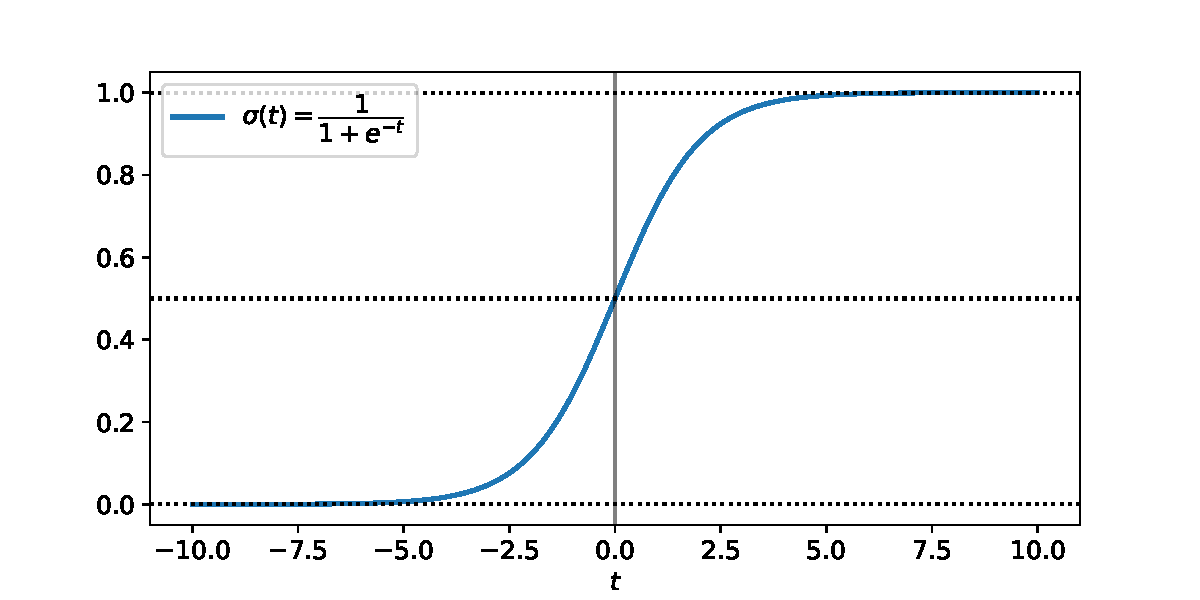
\includegraphics[scale=0.6]{latex/figures/logistic_function.pdf}
\end{center}
\caption{Logistic}
\label{fig:logistic}
\end{figure}

As seen in the figure, the value of the sigmoid function always lies between 0 and 1. The value is exactly 0.5 at $t=0$. Thus, 0.5 can be used as the probability threshold, $p$, to determine the classes. If $p \geq 0.5$ the instance $t$ belongs to the positive class ($y = 1$), or else we classify it as the negative class ($y = 0$).

\textbf{The Logistic Regression Model}

A linear regression model can be represented by

\begin{equation}
    y = \beta^T X
\end{equation}

The logistic regression models estimated probability is then

\begin{equation}
    \hat{p} = \sigma (\beta^T X),
\end{equation}

and the logistic regression model prediction is hence

\begin{equation}
\hat{y} = \begin{cases} 0 \quad \text{if } \hat{p} < 0.5 \\ 1 \quad \text{if } \hat{p} \geq 0.5 \end{cases} 
\end{equation}

\textbf{The Cost Function}

Like for linear regression, we define a cost for our model and the objective will be to minimize the cost.

The cost function of a single training instance can be given by

\begin{equation}
    C(\beta) = \begin{cases} - \log(\hat{p}) &\quad \text{if } y=1 \\ - \log(1-\hat{p}) &\quad \text{if } y=0  \end{cases}
\end{equation}

To show that this cost function makes sense, we plot a simplified version with $t=\beta^T X$ below.

\autoref{fig:logistic_cost}

\begin{figure}[H]
\begin{center}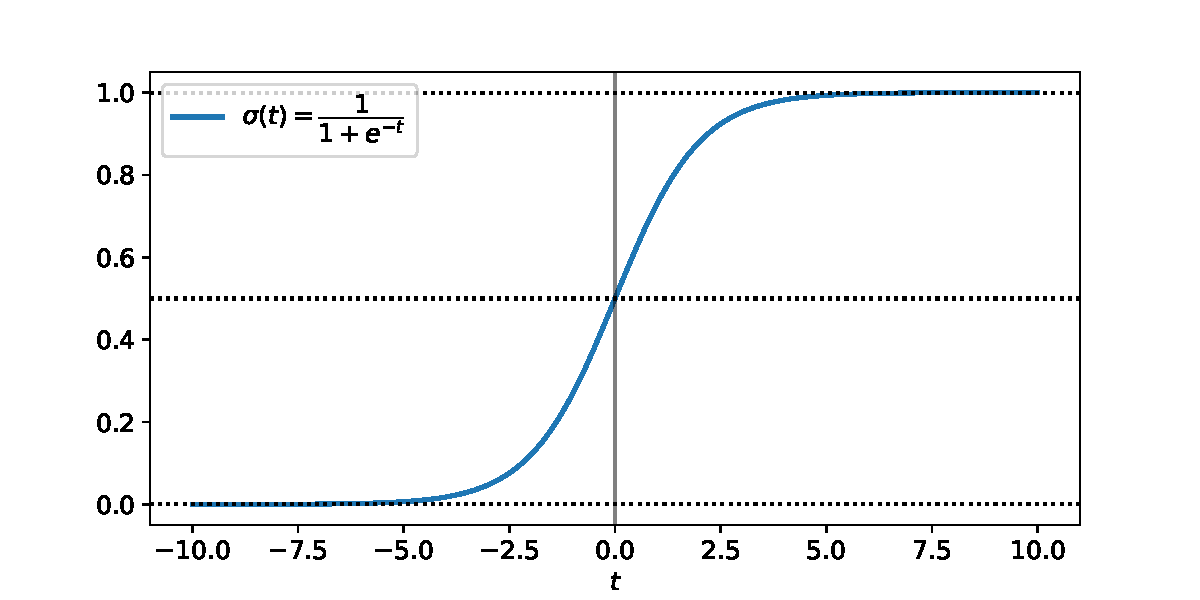
\includegraphics[scale=0.6]{latex/figures/logistic_cost_func.pdf}
\end{center}
\caption{Logistic cost}
\label{fig:logistic_cost}
\end{figure}

The objective of the cost function is to heavily penalize the model if it predicts a negative class ($y=0$) if the acual class is positve ($y=1$) and vice-versa. 

As seen in the above figure, for $C(\beta) = - \log(\hat{p})$ the cost nears 0 as $\hat{p}$ approaches 1 and as $\hat{p}$ nears 0 the cost goes toward infinity (that is, we penalize the model heavily). Similarly, for $C(\beta) = - \log(1 - \hat{p})$, when the actual value is 0 and the model predicts 0, the cost is 0, an the cost goes toward infinity as $\hat{p}$ approaches 1.


%----------------------------------------------------------------
\subsection{Optimization and Gradient Methods}\label{sec:optim theory}
%----------------------------------------------------------------
SGD

Newton-Raphson's method



%----------------------------------------------------------------
\subsection{Neural Network}\label{sec:dnn theory}
%----------------------------------------------------------------



%----------------------------------------------------------------
\subsection{The Ising Model}\label{sec:ising theory}
%----------------------------------------------------------------


\textbf{Excerpt from FYS3150 Project 4}

In statistical mechanics, the Ising model is a model of interacting magnetic dipole moments of atomic spins. The spins, denoted by $S$, are in either a spin up state, with numerical value $+1$ and depicted by $\uparrow$, or a spin down state, with numerical value $- 1$ and depicted by $\downarrow$. The spins are usually arranged in a lattice, where each spin sets up a magnetic field related to the spin direction. This field will decay with the distance from spin $S_i$, so the interaction between spin $S_i$ and $S_j$ will therefore depend on the distance between the spins. As an approximation, the decay of the magnetic field will be assumed to happen rapidly in space, so that the interaction only is between the nearest neighbors \cite[p. 211-212]{Malthe}. A lattice with a specific spin configuration corresponds to a microstate of the system. For $N$ spin particles there are $M=2^N$ possible microstates (or configurations). The energy of a specific configuration $i$ for a system with $N$ spin particles is then given by the Hamiltonian \cite[p. 421]{MHJ}
\begin{equation*}
    H_i = - \sum_{\ev{i,j}}^N J_{ij} S_i S_j - \mathcal{B}_\mathrm{ext} \sum_{j}^N S_j ,
\end{equation*}
where $\ev{i,j}$ indicates that the sum is over the nearest neighbors only, $\mathcal{B}_\mathrm{ext}$ is an external magnetic field interacting with the magnetic moment set up by the spins, and $J_{ij}$ is a coupling constant that includes the effect of the magnetic field set up by spin $i$, the decay of the field with distance, and the coupling between the field and spin $S_j$. In this project, the Ising model is examined without an external field interacting with the lattice, that is, $\mathcal{B}_\mathrm{ext}=0$. Furthermore, all of the nearest neighbors $\ev{i,j}$ is assumed to have the same interaction strength. Thus, the above equation simplifies to
\begin{equation}\label{eq:ising energy}
    E_i = - J \sum_{\ev{i,j}}^N S_i S_j
\end{equation}
For $J>0$ it is energetically favorable for neighboring spins to be aligned. Materials with $J>0$ are ferromagnetic, and exhibit a long-range ordering phenomenon where a given magnetic moment, through interactions between nearest neighbors, can influence the alignment of spins that are separated from the given spin by a macroscopic distance. The appearance of an ordered spin state leads to a phenomenon called spontaneous magnetization, meaning that the lattice has a net magnetization even in the absence of an external magnetic field. However, this property manifest itself only below a critical temperature, called the Curie temperature, $T_C$. For temperatures $T\geq T_C$ the ferromagnetic property disappears as a result of thermal agitation. It is also worth mentioning that the alignment of spins occur within a domain in the material, where different domains will themselves be randomly oriented so that a bulk sample of the material usually is not magnetized \cite[p. 421-422]{MHJ}\cite{HyperPhys}.

In the Ising model, the magnetization is given by \cite[p. 423]{MHJ}
\begin{equation}\label{eq:ising mag}
    \mathcal{M}_i = \sum_{j=1}^N S_j,
\end{equation}
where the sum is over all spins for a given configuration $i$.

\autoref{fig:neighbors} illustrates the concept of “nearest neighbors” in a square lattice in two dimensions, where the spin $S_{i,j}$ sets up a magnetic field which interacts with the neighboring spins $S_{i-1,j}$, $S_{i+1,j}$, $S_{i,j-1}$, and $S_{i,j+1}$.
\begin{figure}[H]
    \begin{minipage}[c]{0.4\textwidth}
    \caption{Neighbors in the the two dimensional Ising model. The neighbors for a spin $S_{i,j}$ are $S_{i-1,j}$, $S_{i+1,j}$, $S_{i,j-1}$, and $S_{i,j+1}$. Figure retrieved from Fig. 7.8 in \cite{Malthe}.} 
    \label{fig:neighbors}
    \end{minipage}\hfill
  \begin{minipage}[c]{0.4\textwidth}
    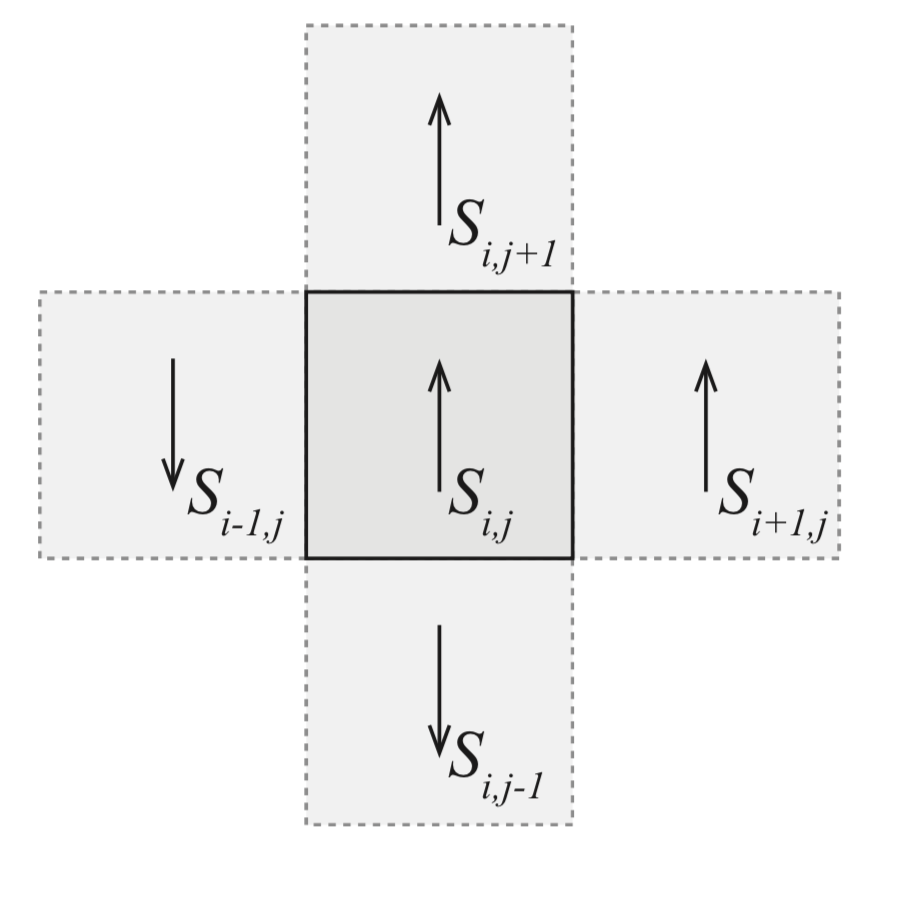
\includegraphics[scale=0.35]{./Images/lattice}
  \end{minipage}
\end{figure}

For the remainder of this project, the magnetic system under consideration will have a ferromagnetic ordering, viz $J>0$. Furthermore, the lattice under consideration will be two dimensional, that is, a square lattice with $L \times L$ spin sites, with $L$ being the number of spins in one dimension.

%----------------------------------------------------------------
\subsection{Periodic Boundary Conditions}\label{sec:pbc theory}
%----------------------------------------------------------------
\textbf{Excerpt from FYS3150 Project 4}

A physical crystal structure consists of a very large number of atoms. In order to model a crystal structure realistically, it usually requires a lattice essentially infinite in all directions. This implies that the behavior of the crystal near the boundaries of the lattice is effectively negligible for the crystal as a whole. It is infeasible to simulate a lattice even remotely approaching a very large number, due to limits of computation. Instead, the boundaries of a relatively small finite lattice must be handled in a manner that ensures a good correspondence with reality. With periodic boundary conditions, spins at the boundary will have its nearest neighbors at the opposite boundary. This ensures that the boundary of a finite lattice has no effect on the behavior of the crystal.
